\documentclass[12pt]{article}

\title{Visualizing the complex Mandelbrot trajectories}
\author{S. Halayka\footnote{sjhalayka@gmail.com}}
\date{\today}

\usepackage{listings}
\usepackage{cite}
\usepackage{xcolor}
\usepackage{graphicx}
\usepackage{setspace}
\usepackage{amsmath}
\usepackage{url}

\usepackage{caption}
\usepackage{subcaption}

%\usepackage[margin=1in]{geometry}
%\doublespace
\begin{document}




\maketitle

\begin{abstract}
The trajectories of the complex Mandelbrot set are visualized using Catmull-Rom curves and OpenGL.
\end{abstract}



\section{Introduction}

As discussed in many papers, books, and websites, a 2D scalar field of complex magnitudes (e.g. $|Z| = \sqrt{Z_x^2 + Z_y^2}$) results from calculating the complex Mandelbrot set when using a finite 2D lattice of regularly spaced vertices as input.
See Figure 1 for the visualization of a lattice.
Iteration is performed to obtain the trajectories of the complex Mandelbrot set.
See Figure 2 for the tiny C++ iteration code.
As shown in Figure 2, the iterative equation is
\begin{equation}
Z = Z^2 + C.
\end{equation}

The criterion for an input location being in the set is that the location's trajectory's end vertex magnitude is always less than some threshold.
See Figure 3 for a low-resolution version of the Mandelbrot set.
For this paper, we use a maximum iteration count of $500$, and a threshold value of $4.0$.

Once all of the complex Mandelbrot set's trajectories have been generated, they are converted to Catmull-Rom curves, to be visualized using OpenGL. 
See Figure 4 for a visualization of some of the complex Mandelbrot trajectories.
See Figure 5 for a medium-resolution version of the Mandelbrot set.

The primary motivation for the exploration of the trajectories of the complex Mandelbrot set was to introduce a new type of visualization: see Figure 6 for all of the complex Mandelbrot trajectories.


\section{Why Catmull-Rom curves?}

Catmull-Rom curves seem to encode a higher degree of fidelity, when it comes to the line passing through all of the control points.
This is unlike B\'ezier curves, where the line is only guaranteed to go through the beginning and end control points.

Catmull-Rom curves offer $C_1$ continuity -- continuity in both position and tangent vectors.
As such, the closed (periodic) loops of the complex Mandelbrot set are easy to visualize.
On the other hand, B\'ezier curves do not offer such built-in $C_1$ continuity.

See Figure 7 for all of the Mandelbrot trajectories, but drawn using Catmull-Rom curves.

See Figure 8 for all of the Mandelbrot trajectories, but drawn using Catmull-Rom curves and pseudorandomly-assigned colours.

Catmull-Rom curves are as computationally intensive as B\'ezier curves, but not much more.

Catmull-Rom curves are attractive-looking.

The quaternion Mandelbrot set is also briefly considered in Figure 9.










\begin{thebibliography}{9}
\bibitem{bourke} Bourke. (2018) ``3D volumetric fractal trajectories''
\bibitem{halayka} Halayka. (2018) ``Visualizing the escape paths of quaternion fractals''
\bibitem{chen} Chen. (2017) ``C++ B\'ezier / spline / Catmull-Rom curve library'' \linebreak \url{https://github.com/chen0040/cpp-spline}

\end{thebibliography}



\pagebreak

\begin{figure} 
\centering
  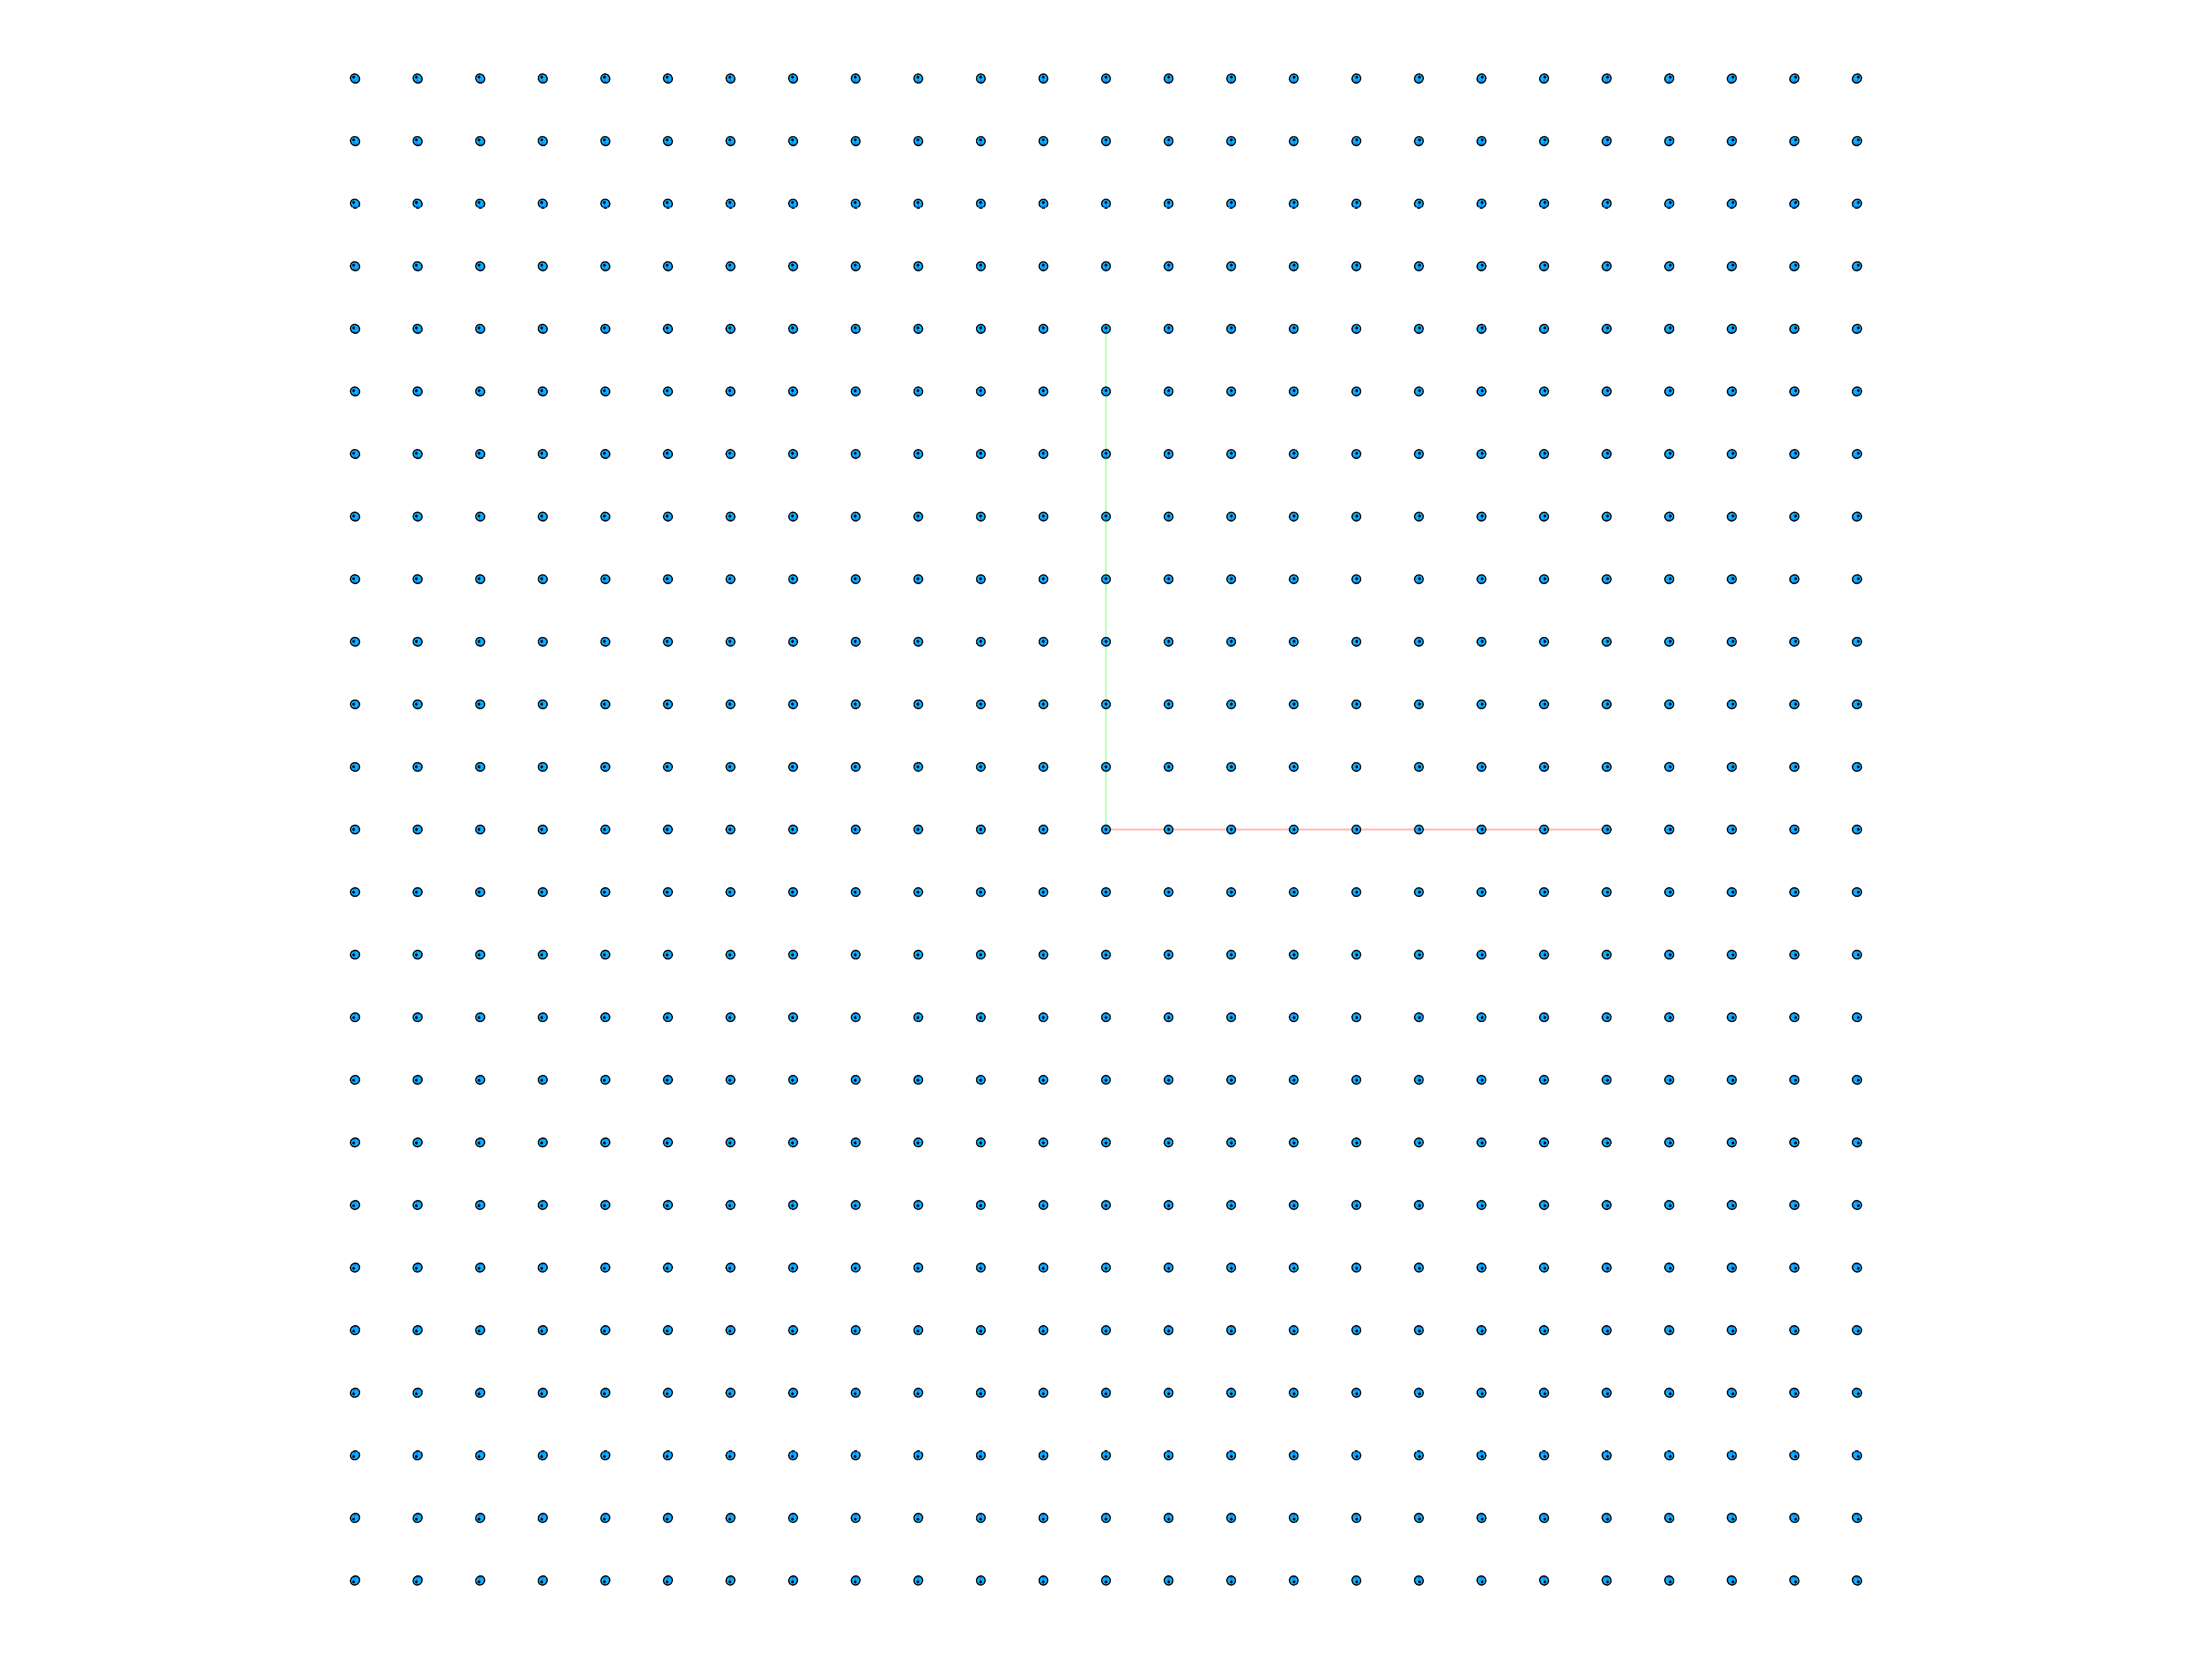
\includegraphics[width = 5 in]{grid.png}	
  \caption{Grid of sample vertices.
Grid minimum = -1.5, grid maximum 1.5.
Resolution = 25.
}
\end{figure}


\begin{figure} 
\centering
  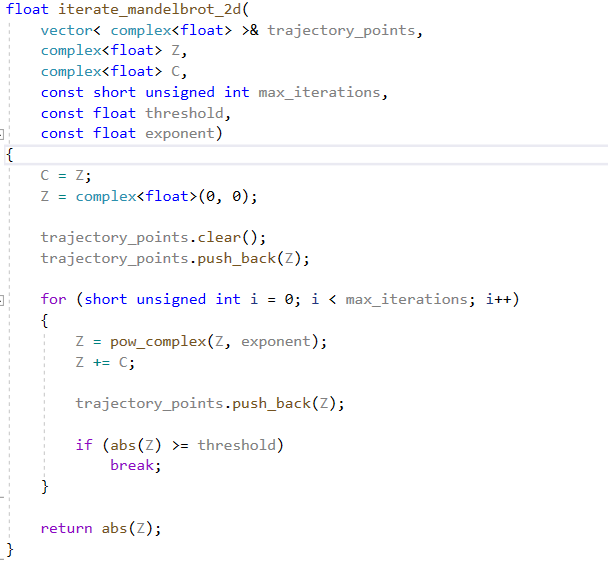
\includegraphics[width = 5 in]{code1.png}	
  \caption{Iteration C++ code.
The exponent is 2.0 for this paper.
}
\end{figure}

\begin{figure} 
\centering
  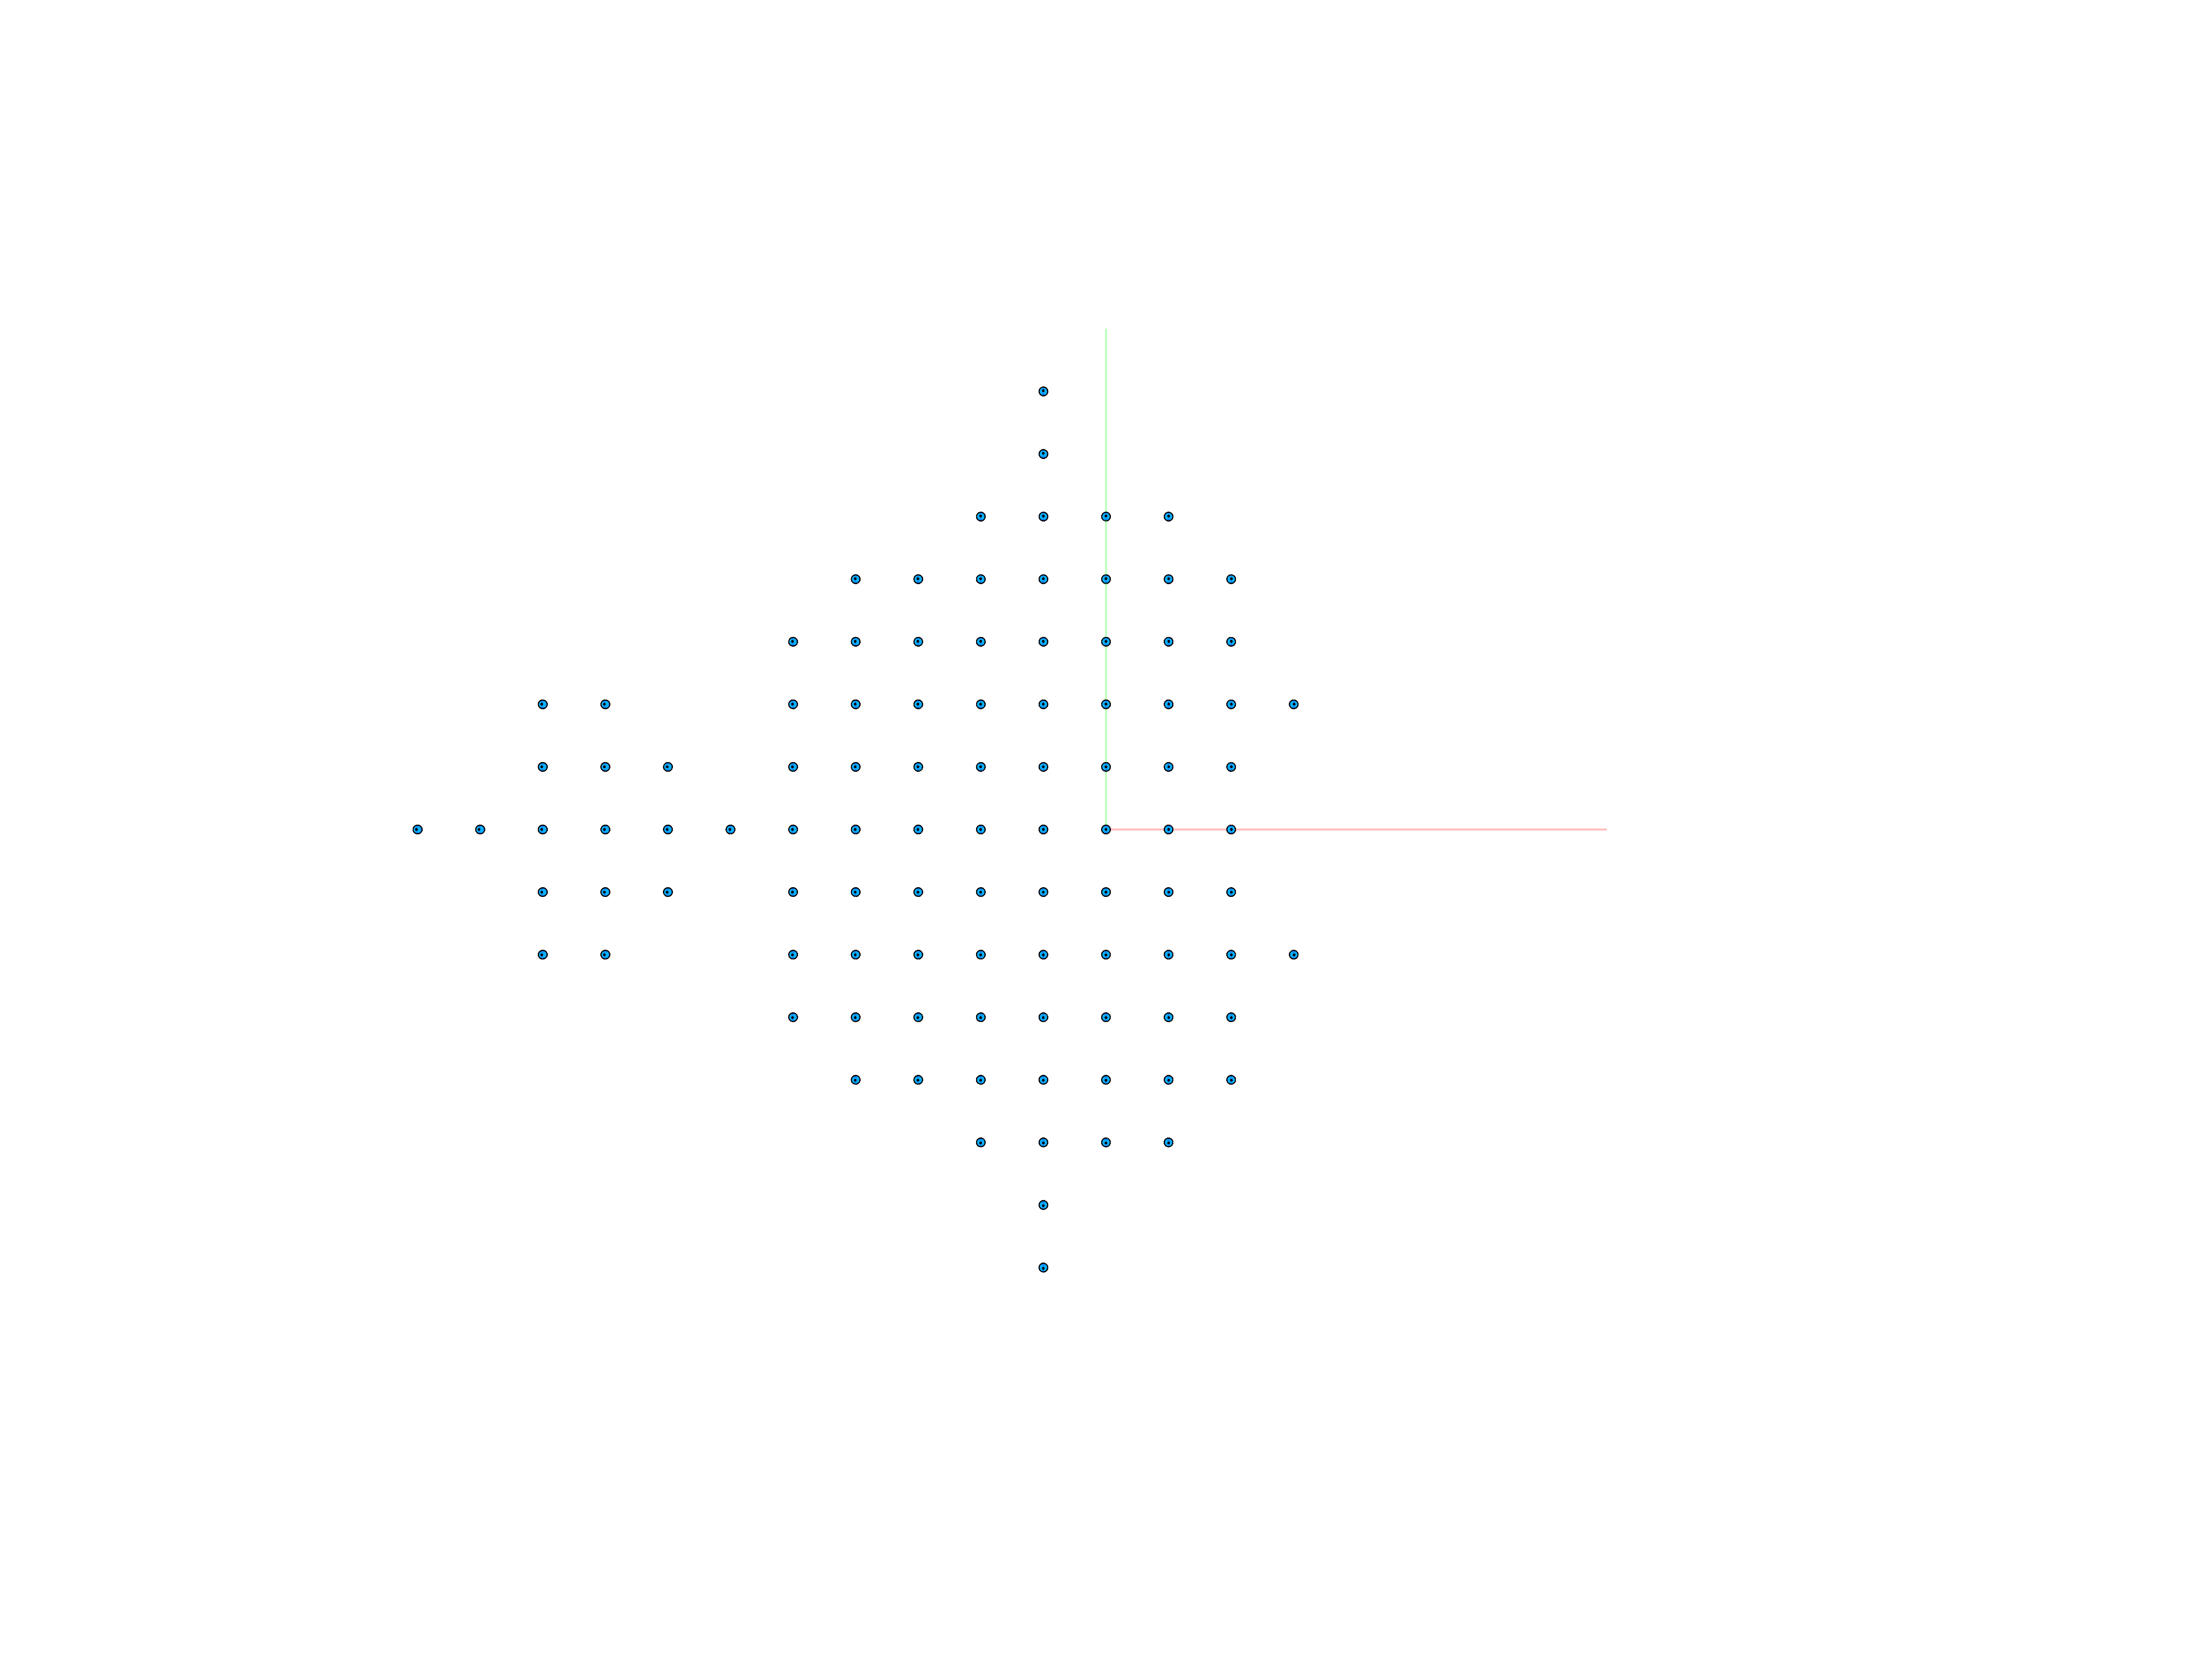
\includegraphics[width = 5 in]{set1.png}	
  \caption{Complex Mandelbrot set.
Maximum iterations = 500.
Grid minimum = -1.5, grid maximum 1.5.
Threshold = 4.0.
Resolution = 25.
No trajectories are drawn.
}
\end{figure}

\begin{figure} 
\centering
  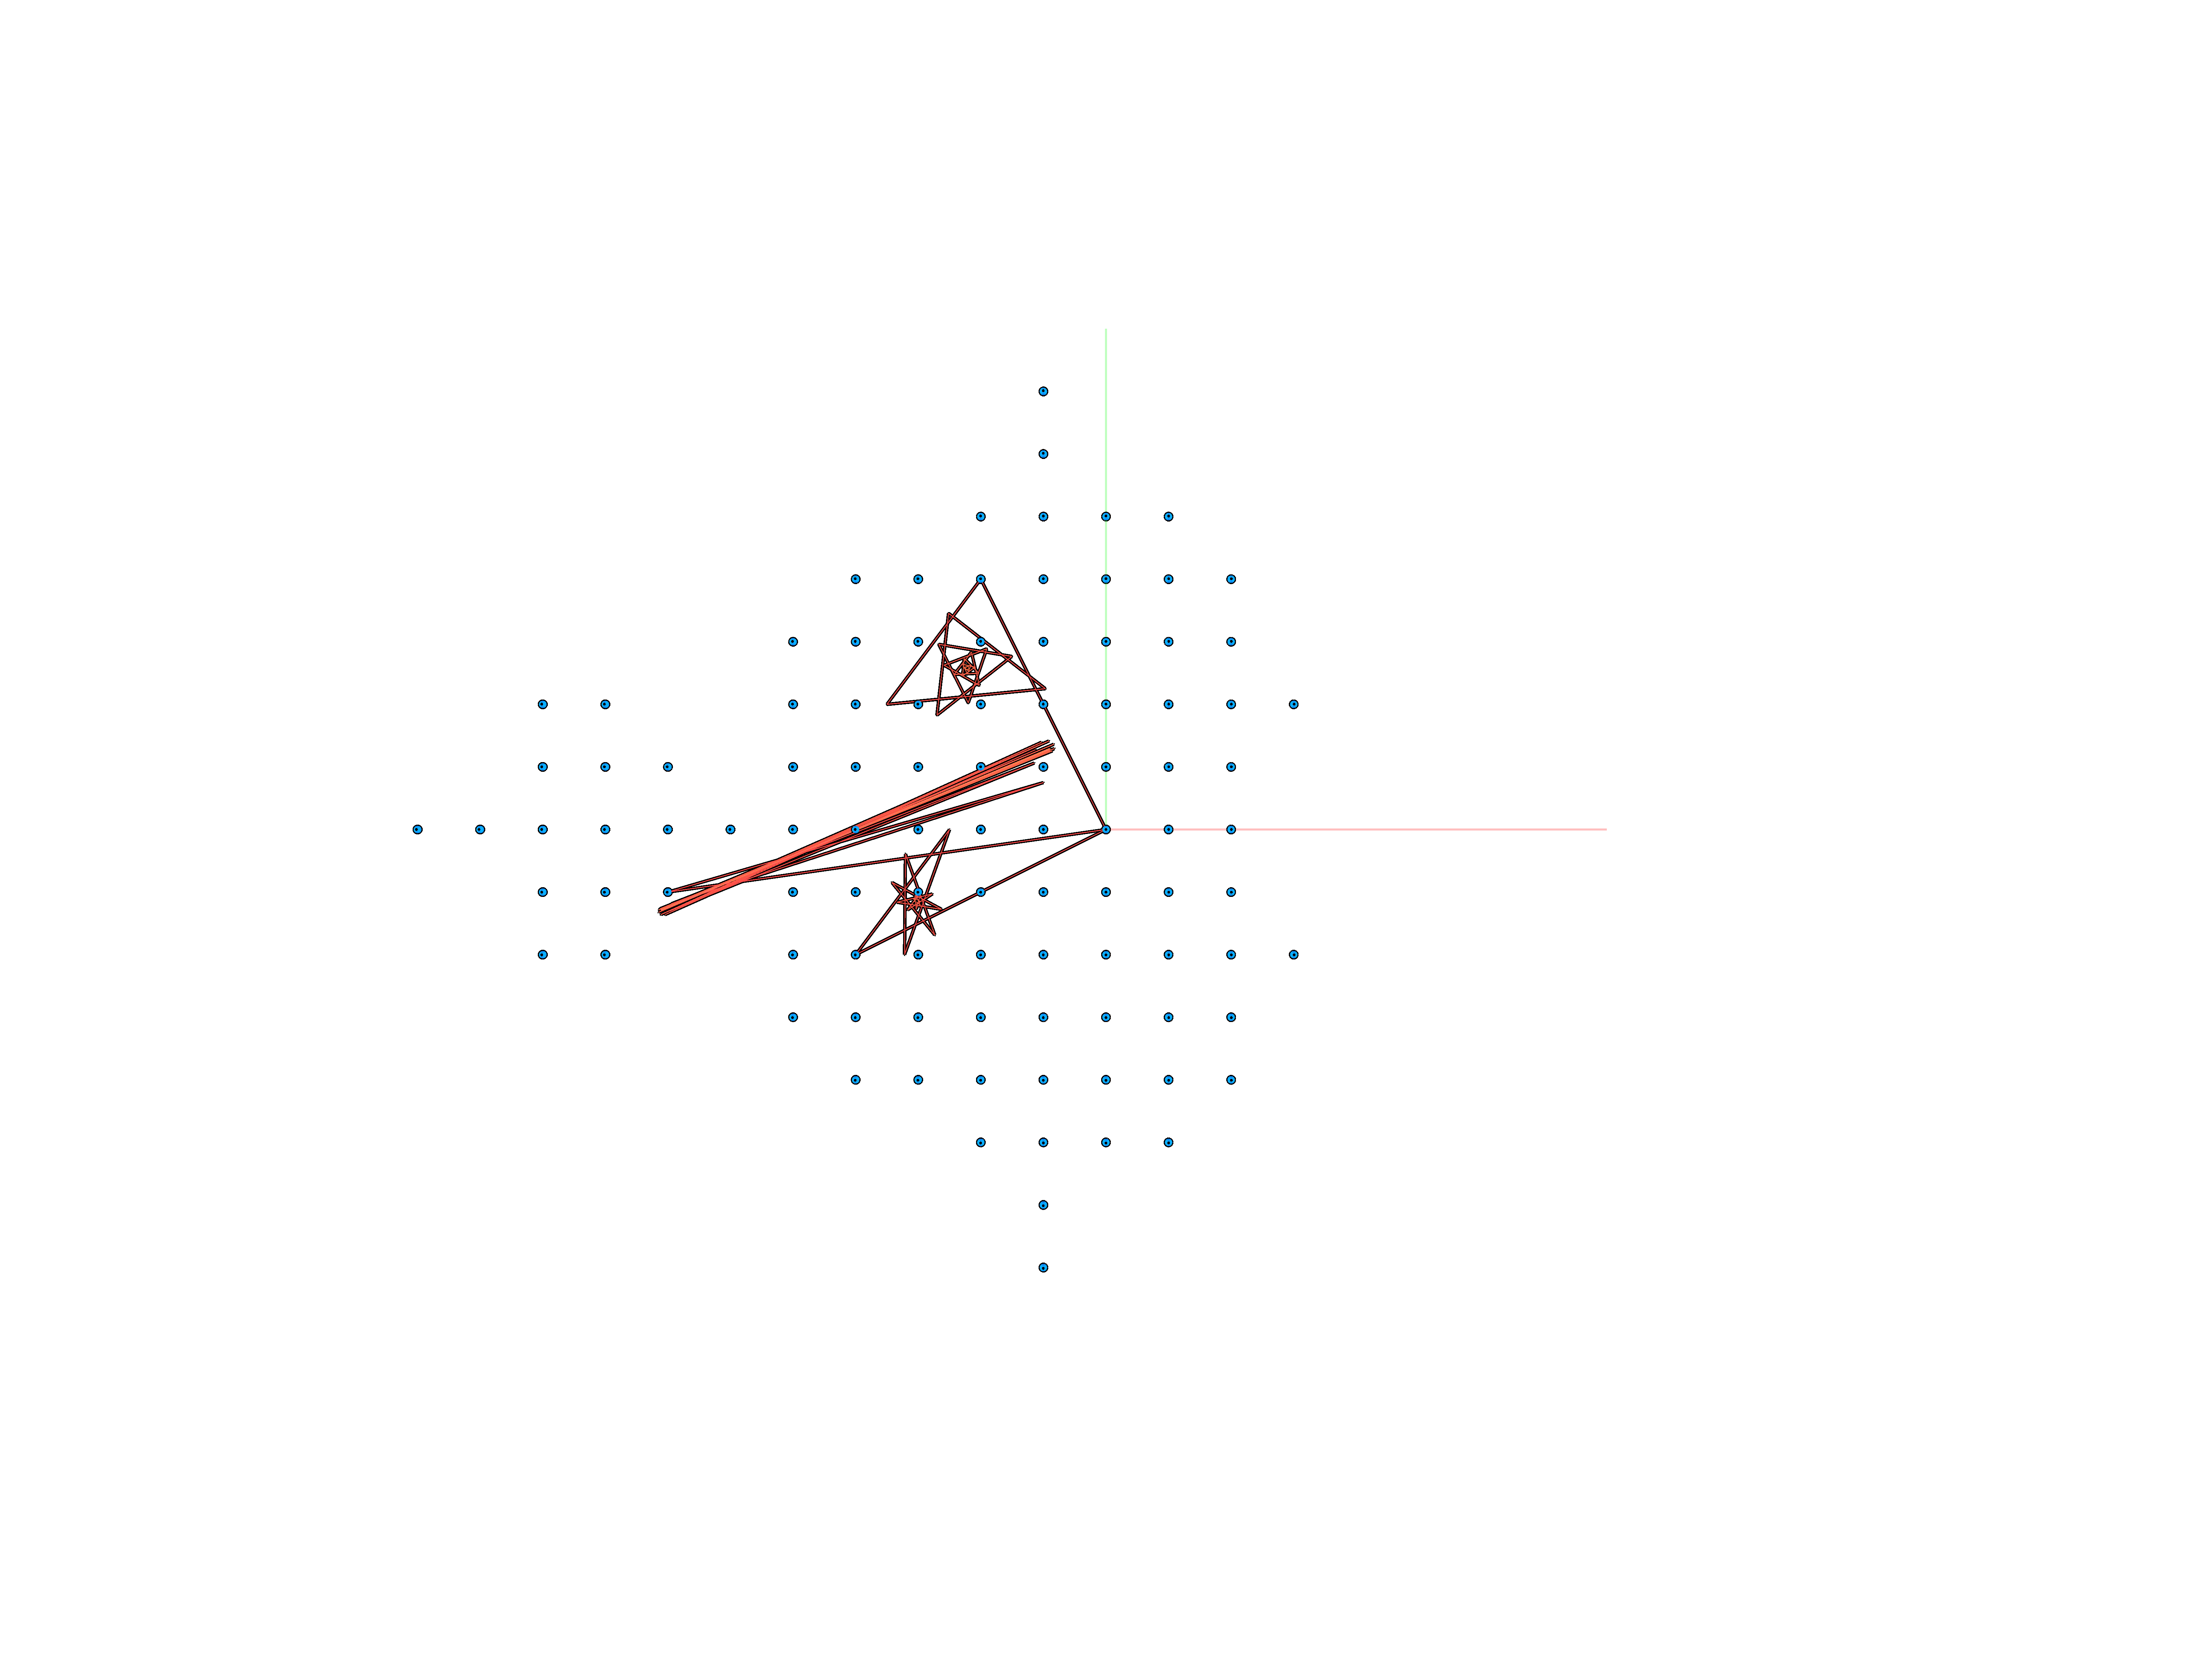
\includegraphics[width = 5 in]{sample_trajectories.png}	
  \caption{A few examples of the complex Mandelbrot trajectories.
Maximum iterations = 500.
Grid minimum = -1.5, grid maximum 1.5.
Threshold = 4.0.
Resolution = 25.
Actual trajectories are drawn.
}
\end{figure}


\begin{figure} 
\centering
  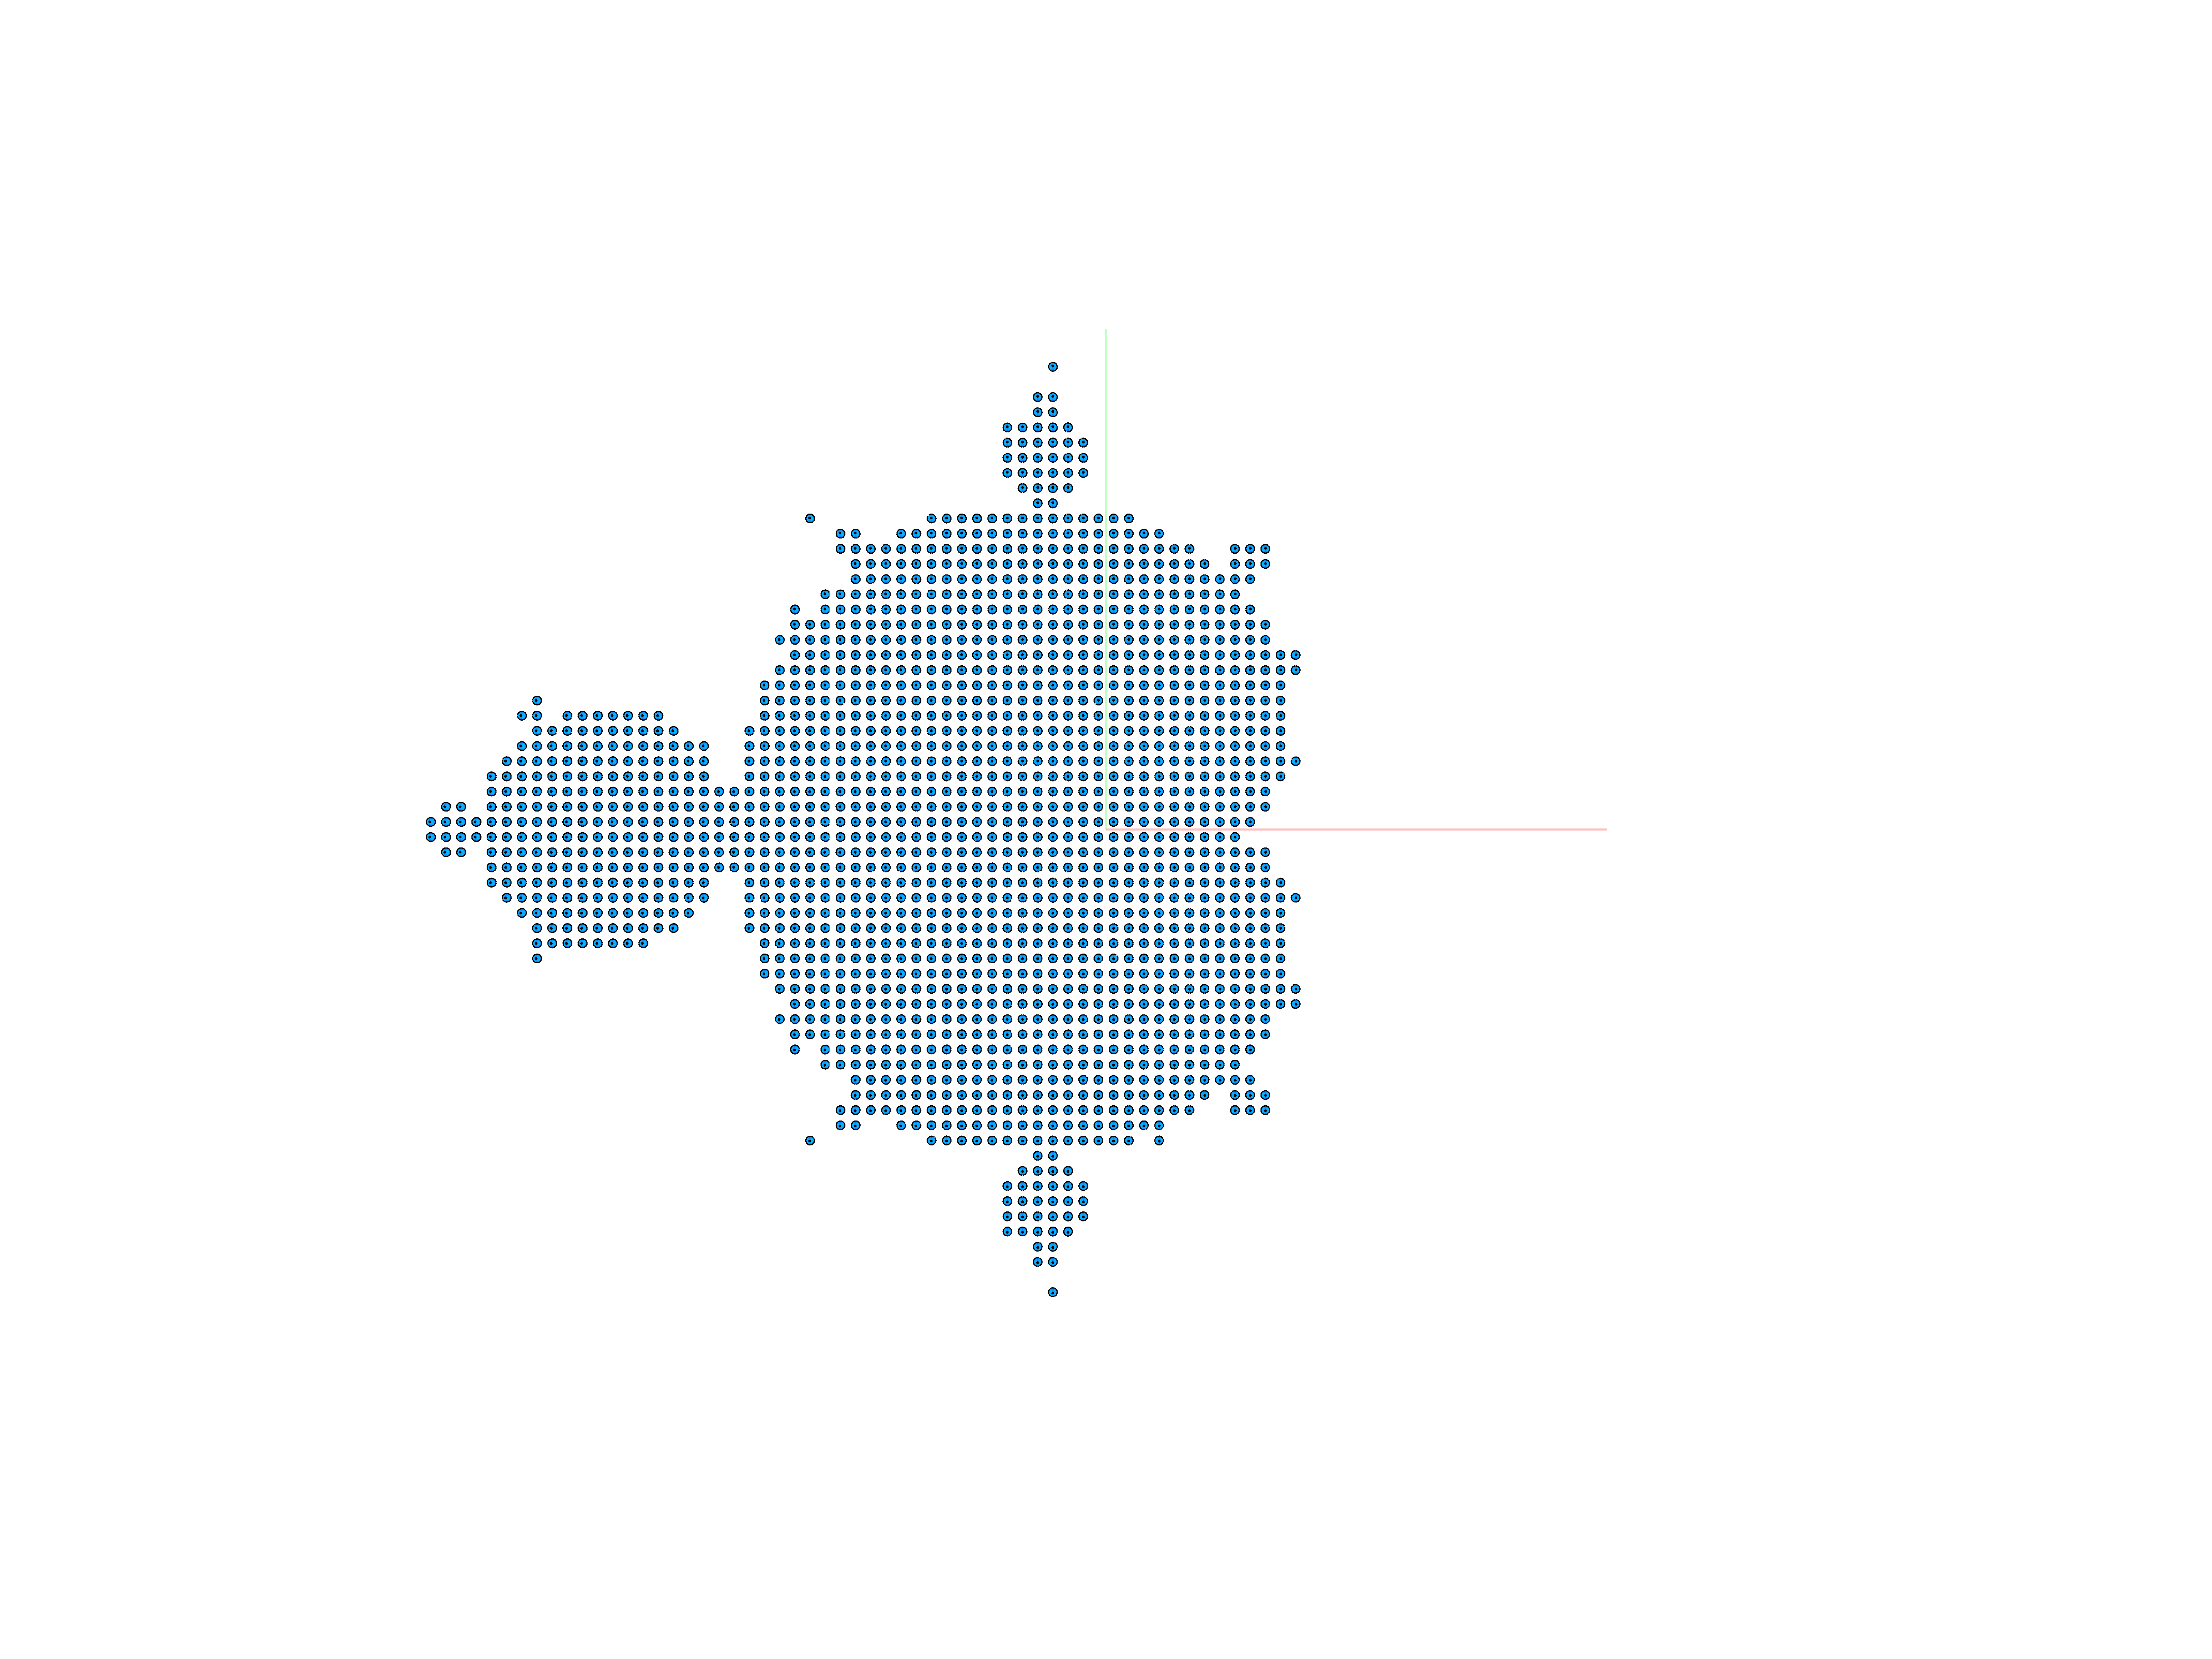
\includegraphics[width = 5 in]{set2.png}	
  \caption{Complex Mandelbrot set.
Maximum iterations = 500.
Grid minimum = -1.5, grid maximum 1.5.
Threshold = 4.0.
Resolution = 100.
No trajectories are drawn.
}
\end{figure}


\begin{figure} 
\centering
  \includegraphics[width = 6.5 in]{rainbow_500_iterations_non_curved.png}	
  \caption{Complex Mandelbrot set.
Maximum iterations = 500.
Grid minimum = -1.5, grid maximum 1.5.
Threshold = 4.0.
Resolution = 25.
Actual trajectories are drawn.
The majority of the trajectories end up being periodic orbits.}
\end{figure}


\begin{figure} 
\centering
  \includegraphics[width = 5 in]{rainbow_500_iterations.png}	
  \caption{
Complex Mandelbrot set.
Maximum iterations = 500.
Grid minimum = -1.5, grid maximum 1.5.
Threshold = 4.0. 
Resolution = 25.
Catmull-Rom trajectories are drawn.
The majority of the trajectories end up being periodic orbits.}
\end{figure}

\begin{figure} 
\centering
  \includegraphics[width = 5 in]{pseudorandom_500_iterations.png}	
  \caption{
Complex Mandelbrot set.
Maximum iterations = 500.
Grid minimum = -1.5, grid maximum 1.5.
Threshold = 4.0.
Resolution = 25.
Catmull-Rom trajectories are drawn.
Pseudorandomly-assigned colours are used, to help differentiate between the individual trajectories.
The majority of the trajectories end up being periodic orbits.}
\end{figure}


\begin{figure} 
\centering
  \includegraphics[width = 5 in]{quaternion_mandelbrot.png}	
  \caption{
Quaternion Mandelbrot set.
Maximum iterations = 500.
Grid minimum = -1.5, grid maximum 1.5.
Threshold = 4.0.
Resolution = 10.
Catmull-Rom trajectories are drawn.
As is with the complex Mandelbrot set, the majority of the quaternion Mandelbrot trajectories end up being periodic orbits.}
\end{figure}


\end{document}









